\DiaryEntry{Poisson Process, 2}{2019-04-04}{Stochastic}

Now assume that we observe a Poisson process and within a time interval $t$ there are $n$ arrivals. Based on this observation, we want to obtain the ML estimate $\hat\lambda$ for $\lambda$.

We start with the PMF for $N(t)$ (Poisson distribution),

\bee
f_{N(t)}(n) = \frac{(\lambda t)^n e^{-\lambda t} }{ n!  }
\eee

For completeness, we have plotted the PMF as function of $n$ for values of $\lambda = 3, 7, 10$ and fixed $t=1$ in the Figure below.

\begin{figure}[H]
  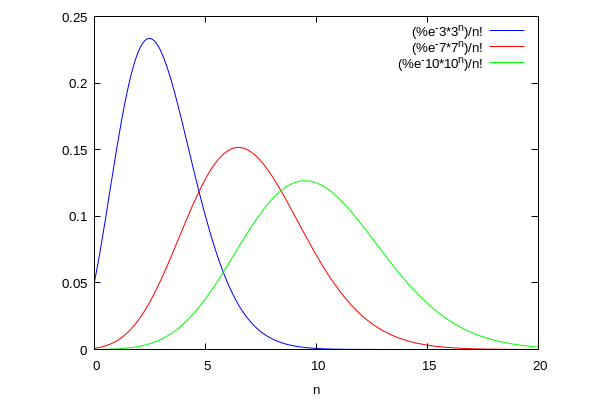
\includegraphics[scale=0.6]{images/poisson_process_2_1.png}
\end{figure}


To get an ML estimator, we differentiate the PMF with respect to $\lambda$ and set it to zero.

\bee
\frac{\partial f_{N(t)}(n)}{\partial \lambda} = \frac{t^n}{n!} \left( n \lambda^{n-1} e^{-\lambda t} - t \lambda^n e^{-\lambda t} \right)
\eee

Setting this to zero yields

\bee
n \lambda^{n-1} e^{-\lambda t} - t \lambda^n e^{-\lambda t} = 0 \rightarrow n - t \lambda = 0
\eee

and finally the ML estimate

\bee
\hat \lambda = \frac{n}{t}
\eee

When we interpret $\lambda$ as the mean of interarrival times, the ML estimate is the number of arrivals per time interval, which makes intuitively sense. The Figure below shows the PMF as function of $\lambda$ for n=$5,10$ and fixed $t=1$.


\begin{figure}[H]
  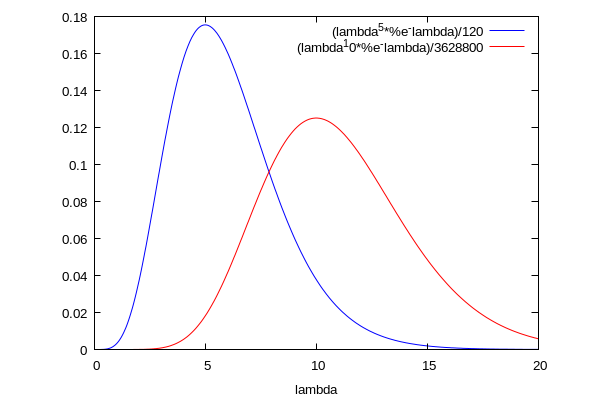
\includegraphics[scale=0.6]{images/poisson_process_2_2.png}
\end{figure}

\todo{What happens in case $n=0$?}


%%% Local Variables:
%%% mode: latex
%%% TeX-master: "journal"
%%% End:
